\documentclass{article}
\usepackage{gensymb}
\usepackage{lstlinebgrd}
\usepackage{graphicx}
\graphicspath{ {./res-images/} }

\begin{document}

\title{Building Resilience Vaccine Distribution}
\author{Saransh Sharma }
\date{January 2021}


\maketitle

\section{Introduction}

Vaccine in India is approved for restricted use in emergency situation in public interest as an abundant precaution, in clinical trial mode, especially in the context of infection by mutant strains.\footnote{https://www.bbc.com/news/world-asia-india-55534902}, though there are serious concerns on lack of evidence and unsatisfactory scientific evidence for the vaccine produced in India.\footnote{bae2020challenges}

Planning for country wide operations has already begun, for now frontline workers and people in need like age above 50 with pre-conditions will receive vaccine first. Current situation of infection across globe stands at 37.3 M, 10M+ in India. COVID-19 amounts to 149K death in India alone.
Government of India has launched COWIN program\footnote{https://pib.gov.in/PressReleasePage.aspx?PRID=1683001} to strengthen vaccine intelligence, this open call is for partners to provide answers to 7 key problems identified by government.

Before building a strong vaccine intelligence network that provides last mile delivery to the one in need there needs a strong focus on filling the gaps in distribution. The world’s manufacturing processes and supply chains are underprepared for the task of widespread vaccine distribution\cite{bae2020challenges}.Movement of vaccine in India posses challenges of unknown and unresolved issues that can cause delay. To be able to implement at scale key challenges of maintaining stable temperature ie cold chain , current capacity of cold chain is inadequate for existing vaccination programs\footnote{https://www.bloombergquint.com/global-economics/india-faces-cold-chain-logistics-challenge-for-virus-vaccination}. WHO recommends vaccine should be stored at 2-8\degree C, but studies showing vaccines are exposed to temperature above 8 \degree C\cite{dhere2011pandemic} at every level of storage as vaccine cross different regions. Hence, Coordinated efforts between regional level needed to achieve a stable cold chain with an alternative approach that can offset the waste of vaccine.

Recording data at sites of users by healthcare worker is critical, studies has shown that 10-60\% of data is inaccurate\cite{atkinson2020digital}}. Several challenges like what kind of data is recorded when administering vaccine still persist. Finding solutions and alternative interfaces to record data to reduce inaccuracy. Utilising that data for managing validation across the information system. Data management across different level of local, regional and state. This data could be used across different verticals to make descions.

In this paper we define different approaches and practical solutions to certain problems we have identified by reviwing literature. We have defined these solutions in 

\begin{enumerate}
	\item Synchronicity
	\item Event Layer
	\item AI For Finding Locations
	\item Cold Chain Alternative
	\item Use of Cryptographic Methods
\end{enumerate}




\section{Synchronicity}
In order to capture and utilise data from different verticals it is important to implement synchronous data layer that keeps updating data in real time. There are going to be variety of services that is going to create data attributes. A service that interacts with VIN sends a message , that passes through a parser and goes to the receiving end. This whole process can be stored as message streams or log for various auditable purpose later. This process is known as event sourcing , services recording all the states together as a sequence of events, this kind of design allow to reconstruct past states. Its quite straightforward and less consuming than querying database.

Implementing an indexer that identifies what kind of attributes are most frequently used , those attributes can be stored as meta-data. This meta-data can be used as a template when a service is sending out a message. For an eg: At a clinic when frontline worker recording data about vaccine, they could use the metadata rather then pre-defined field. This meta-data is useful in terms of what kind of attributes is important from different verticals.

General steps of the building a sync layer is to have a Parser, the job of a parser is to clean data, after messages gets through parser validating data. The major goal of this layer is to reduce friction and establish communication between working groups and services.

Practical Application such as RFID, sensors, Applications collecting data from delivery points, logistics and supply chain instrument that will create data at different vectors.

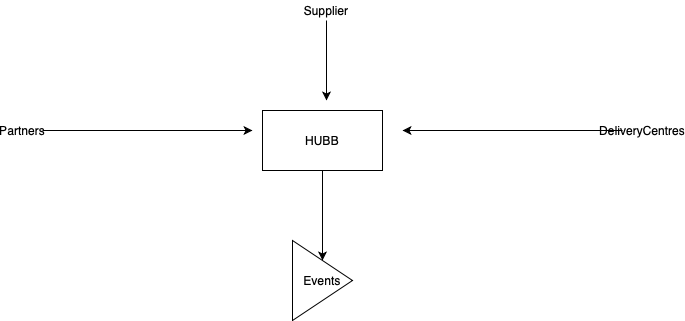
\includegraphics[scale=0.5]{hubb}


\begin{lstlisting}
	createData()
	parseData()
	processData()
		identify()
		extract()
		reshape()
	return()	
\end{lstlisting}

   
\section{Eventing Layer}

A process that involves sending out important alerts and notices	, eventing layer comes in place. The overall use of  layer is to identify and sends notices and warnings to the interested parties and services that are involved in a process. A process could be like delivering vaccines to users, shipping vaccines from a location. All of these processes have pre-defined steps and in case of deviation of these step eventing layer should send out notifications to involved parties.

One example is to use this service to manage end to end shipping and defining events points, these points can be flow, or logical steps, or an incident. When any incident is triggered at any level, parties are notified. Practical example, vaccine supply reaches with tampered unit, notices and alerts reaching to vaccine delivery site and the one who delivered.

This eventing layer can use the above data layer to identify parameters from data attributes, like when to send notification, who to send like who are parties. This kind of eventing layer is already available in modern web-apps these days specifically in machine learning.

\section{AI}
AI is a powerful catalyst today, the use of AI in healthcare is quite visible such as  drug discovery. Scientist are using inexpensive and rapid implementation for finding therapies, if given enough data it can aid the search of the drug\cite{keshavarzi2020artificial}. Once we have built the information that allow us to have quality data with few errors, we could use sophisticated math models and to train them using re-inforcement learning. Hence machine could be trained and  help in predictions for forecasting inventory, preparing for hazard , analysing the turn around time based on the overall supply chain optimal functioning. We describe these models here that can be fed in any application to achieve optimal distribution.

\begin{enumerate}
	\item Present vaccine distribution largely focus on individual at risk, We can use spatiotemporal regions with the most new cases of infection during a certain time frame and compare it with the standard practice of distributing vaccines demographically. A computational model presented in\cite{grauer2020strategic} , for a locally well-mixed population,strongly reduces the number of deaths by 35\%. This model purely puts emphasis on density of the population on a given space and time ie a region, targeting using a math based model and realising herd immunity.
	\item Typically vaccines are distributed via a four-tier hierarchical networks, classic WHO-EPI model inherently is limited to meeting the demand, fixing location of the clinic. Mixed integer programming solves key issues of selecting storage sizes and ensures all delivery is made in single trip\cite{yang2020optimizing}. This model is based on hubs, nodes associated to these hubs. Below table shows the numerical output using MIP model.
  
	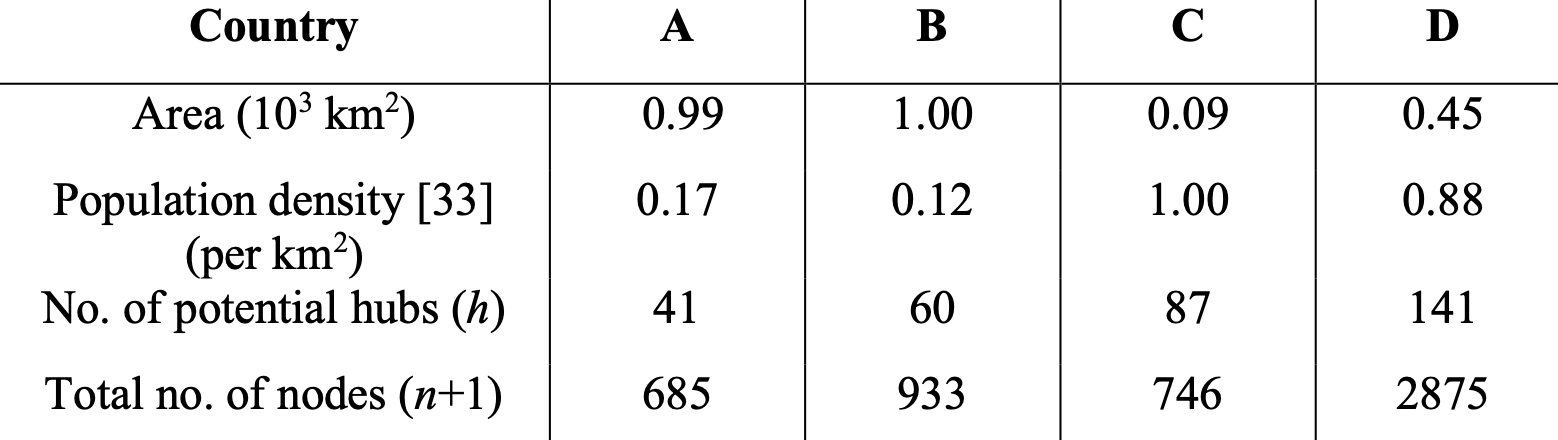
\includegraphics[scale=0.4]{maths.png}
	\item Since real world experimentation is out of question , there are unknown problems that can occur, scarcity of vaccine or sub-components. Resulting dynamics may change over time, enough data supplied with contextual policies with demographics for the fair distribution. VacSim model emphasis challenges that need solving in real time, with no ground truth availability. This model employs classic re-inforcement learning with forward feed that can be optimised in real time.\cite{awasthi2020vacsim}

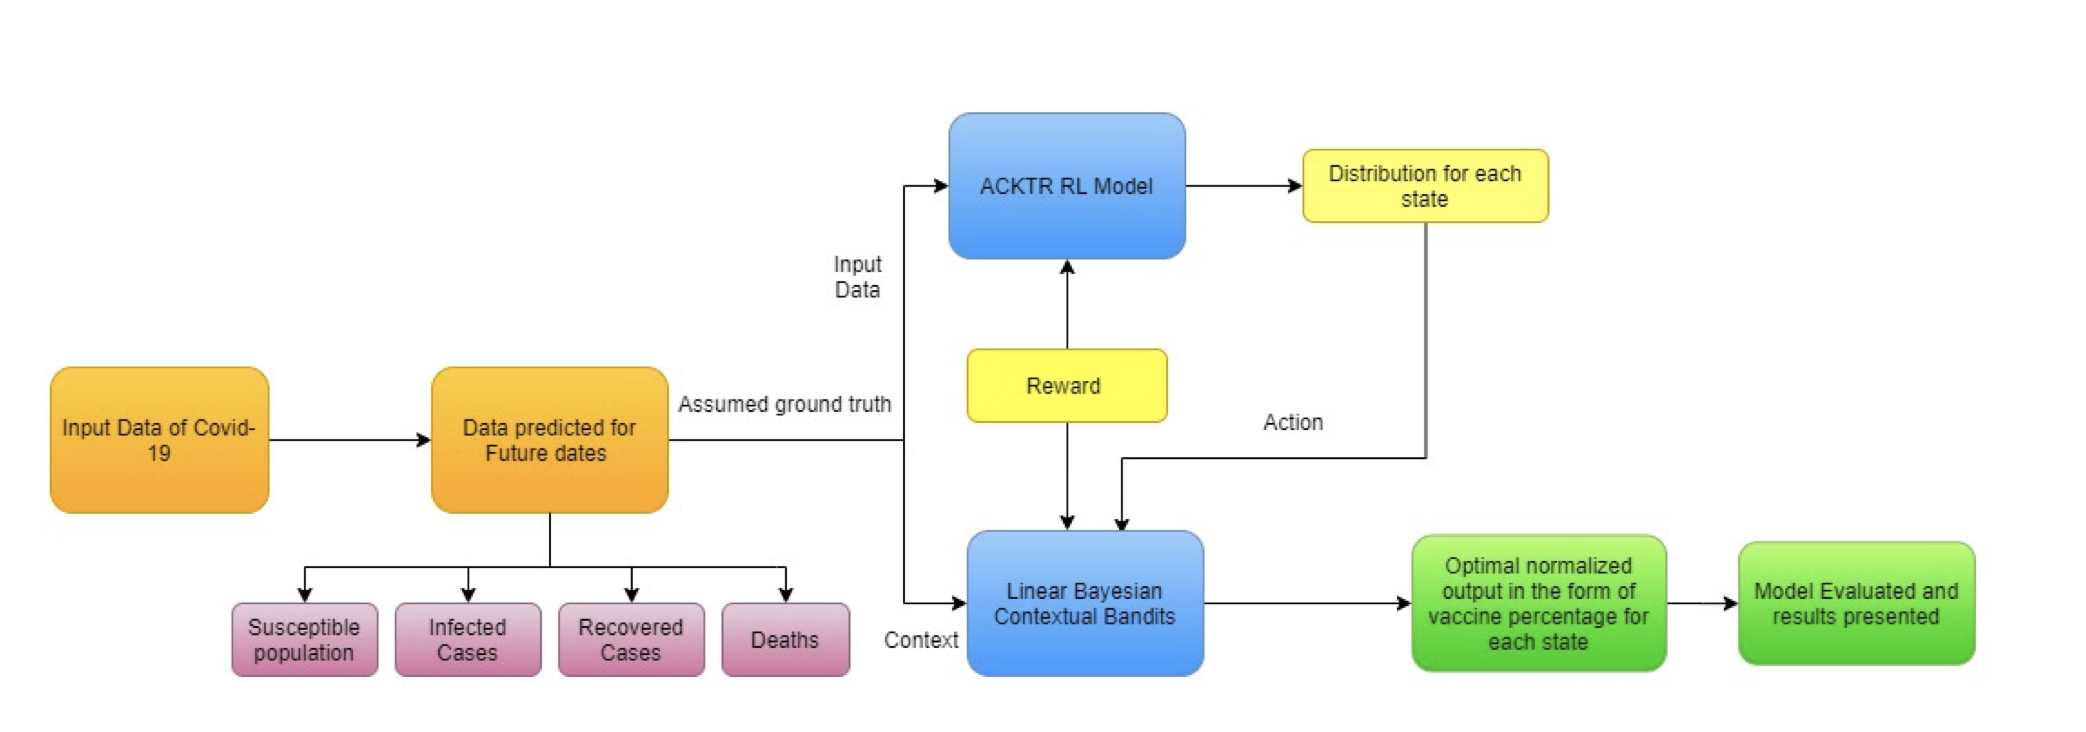
\includegraphics[width=\textwidth]{model.png}
	\item 

\end{enumerate} 
 

\section{Cold Chain Alternative}

There are cold chain alternative

\section{Cryptographic Methods}
	

  


\bibliographystyle{aabbrv}
\bibliography{bib/graph}


\end{document}




